\documentclass[border=4pt]{standalone}
 
\usepackage{mathpazo}
\usepackage{pgfplots}
\newcommand{\num}{pi}
\pgfplotsset{compat=1.8}

 % define the plot style and the axis style
\tikzset{elegant/.style={smooth,thick,samples=50,magenta}}
\tikzset{
    between/.style args={#1 and #2}{
         at = ($(#1)!0.5!(#2)$)
    }
}
\usetikzlibrary{calc}
\usetikzlibrary{positioning}
 
\begin{document}

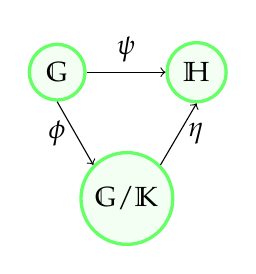
\begin{tikzpicture}[
roundnode/.style={circle, draw=green!60, fill=green!5, very thick, minimum size=7mm},
%squarednode/.style={rectangle, draw=red!60, fill=red!5, very thick, minimum size=5mm},
]
%Nodes
%\node[squarednode]      (maintopic)                              {2};
\node[roundnode]        (uppercircle1)                                         {$\mathbb{G}$};
\node[roundnode]        (uppercircle2)      [right = of uppercircle1] {$\mathbb{H}$};
\node[roundnode]        (lowercircle)       [below = of uppercircle1, between= uppercircle1 and uppercircle2] {$\mathbb{G} /\mathbb{K}$};

%Lines
\draw[->] (uppercircle1.east) -- (uppercircle2.west) node[midway,above] {$\psi$};
\draw[->] (uppercircle1.south) --(lowercircle.north west) node[midway,left] {$\phi$}; ;
\draw[->] (lowercircle.north east) -- (uppercircle2.south) node[midway,right] {$\eta$};;
\end{tikzpicture}
 
\end{document}